% ******************************************************** %
%              TEMPLATE DE INFORME ORGA2 v0.1              %
% ******************************************************** %
% ******************************************************** %
%                                                          %
% ALGUNOS PAQUETES REQUERIDOS (EN UBUNTU):                 %
% ========================================
%                                                          %
% texlive-latex-base                                       %
% texlive-latex-recommended                                %
% texlive-fonts-recommended                                %
% texlive-latex-extra?                                     %
% texlive-lang-spanish (en ubuntu 13.10)                   %
% ******************************************************** %


\documentclass[a4paper]{article}
\usepackage[spanish]{babel}
\usepackage[utf8]{inputenc}
\usepackage{charter}   % tipografia
\usepackage{graphicx}
%\usepackage{makeidx}
\usepackage{paralist} %itemize inline
\usepackage{subcaption}


%\usepackage{float}
%\usepackage{amsmath, amsthm, amssymb}
%\usepackage{amsfonts}
%\usepackage{sectsty}
%\usepackage{charter}
%\usepackage{wrapfig}
%\usepackage{listings}
%\lstset{language=C}

% \setcounter{secnumdepth}{2}
\usepackage{underscore}
\usepackage{caratula}
\usepackage{url}
\usepackage{ragged2e}
\usepackage{hyperref}
\usepackage{pdfpages}


% ********************************************************* %
% ~~~~~~~~              Code snippets             ~~~~~~~~~ %
% ********************************************************* %

\usepackage{color} % para snipets de codigo coloreados
\usepackage{fancybox}  % para el sbox de los snipets de codigo

\definecolor{litegrey}{gray}{0.94}

\newenvironment{codesnippet}{%
	\begin{Sbox}\begin{minipage}{\textwidth}\sffamily\small}%
	{\end{minipage}\end{Sbox}%
		\begin{center}%
		\vspace{-0.4cm}\colorbox{litegrey}{\TheSbox}\end{center}\vspace{0.3cm}}



% ********************************************************* %
% ~~~~~~~~         Formato de las páginas         ~~~~~~~~~ %
% ********************************************************* %

\usepackage{fancyhdr}
\pagestyle{fancy}

%\renewcommand{\chaptermark}[1]{\markboth{#1}{}}
\renewcommand{\sectionmark}[1]{\markright{\thesection\ - #1}}

\fancyhf{}

\fancyhead[LO]{Sección \rightmark} % \thesection\ 
\fancyfoot[LO]{\small{Ivo Pajor, Laureano Muñiz, Luciana Gorosito}}
\fancyfoot[RO]{\thepage}
\renewcommand{\headrulewidth}{0.5pt}
\renewcommand{\footrulewidth}{0.5pt}
\setlength{\hoffset}{-0.8in}
\setlength{\textwidth}{16cm}
%\setlength{\hoffset}{-1.1cm}
%\setlength{\textwidth}{16cm}
\setlength{\headsep}{0.5cm}
\setlength{\textheight}{25cm}
\setlength{\voffset}{-0.7in}
\setlength{\headwidth}{\textwidth}
\setlength{\headheight}{13.1pt}

\renewcommand{\baselinestretch}{1.1}  % line spacing

% ******************************************************** %


\begin{document}


\thispagestyle{empty}
\materia{Organización del Computador II}
\submateria{Segundo Cuatrimestre de 2020}
\titulo{Trabajo Práctico III}
\subtitulo{System Programming}
\integrante{Ivo Pajor}{460/19}{ivo_pajor@hotmail.com}
\integrante{Laureano Muñiz}{498/19}{lau2000m@hotmail.com}
\integrante{Luciana Gorosito}{577/18}{lugorosito0@gmail.com}

\maketitle


\thispagestyle{empty}
\vfill


\thispagestyle{empty}
\vspace{3cm}
\tableofcontents
\newpage


%\normalsize
\newpage

\section{Introducción}
\justify
El objetivo de este trabajo práctico es aplicar gradualmente los conceptos de \textit{System Programming} vistos en las clases teóricas y prácticas, mediante la implementación de una serie de ejercicios que, inspirados en la serie \textit{Rick y Morty}, en conjunto conformarán un kernel o un pequeño sistema operativo.



\section{Desarrrollo}
\justify
A continuación detallamos las implementaciones de los ejercicios del trabajo práctico.

\subsection{Ejercicio 1}
\justify
Para la realización de este ejercicio analizamos las estructuras \textbf{gdt_entry_t} y \textbf{gdt_descriptor_t} definidas por la cátedra. En esta implementación, la Tabla de Descriptores Globales(GDT) es un arreglo de  \textbf{gdt_entry_t} y su descriptor, que luego cargaremos en GDTR, es del tipo \textbf{gdt_descriptor_t}.\par
\justify
Siguiendo lo indicado en el primer item, definimos a partir del índice 10, 4 descriptores de segmento en la GDT utilizando la estructura \textbf{gdt_entry_t}, atendiendo a las propiedades particulares de cada segmento. Así definimos las entradas de dos segmentos de código de nivel
0 y 3 y de dos segmentos de datos, también de nivel 0 y 3. Puesto que estos segmentos deben direccionar los primeros 201 MB de memoria establecimos en todos el bit de G en 1, y definimos su base en 0x00000000 y su limite en 0x00C8FF. Además, como son segmentos de código o datos de 32 bits, los bit S y D/B se encuentran seteados en 1 y el bit L en 0. Los bits de DPL de cada uno están seteados en 0 o en 3 de acuerdo con el nivel de privilegio que le corresponda. Por último, los bits de tipo están seteados como 0xA en caso de tratarse de un segmento de código y como 0x2 en caso de tratarse de un segmento de datos. En todos, el bit P se setea en 1 para reflejar que los segmentos están presentes. En el caso del bit de AVL, como es un bit reservado lo seteamos en 0.

\begin{figure}[h]
	\centering
	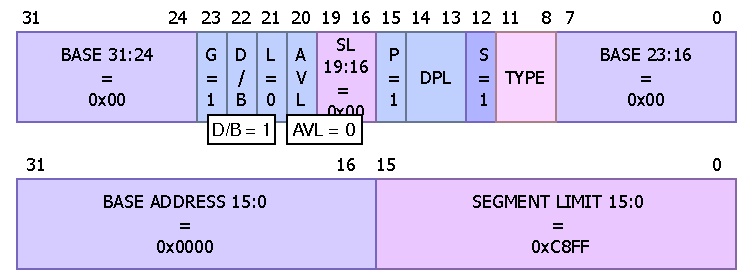
\includegraphics[scale=0.8]{img/GDTdescriptor.pdf}
	\caption{Esquema general de un descriptor de la GDT para los 4 segmentos.}
\end{figure}


\justify
Realizando lo pedido en el item b, pasamos a modo protegido. Para poder hacer esto modificamos el archivo kernel.asm, allí deshablitamos las interrupciones, cargamos en el registro GDTR la estructura \textbf{gdt_descriptor_t} y modificamos el ultimo bit del registro de control CR0, es decir, seteamos en 1 el bit de \textit{Protection Enable}. Posteriormente, escribimos el código necesario para saltar efectivamente a modo protegido. Debido a que este salto se consigue haciendo un \textit{far jump} a la próxima instrucción, designamos una etiqueta llamada \textbf{modo_protegido} a partir de la cual obtendremos el offset, mientras que como selector utilizamos el correspondiente al segmento de código de nivel 0. Además, seteamos la pila del kernel en la dirección 0x25000, es decir, en la base de la pila. Una vez que pasamos a modo protegido, cargamos correctamente los selectores de segmento, en los registros ds, es, fs, gs, ss, usando como registro auxiliar ax.


\justify
Seguidamente, definimos otra entrada en la GDT destinada a un segmento de vídeo. A diferencia de los cuatro segmentos anteriores, la base de este segmento es distinta de 0, por lo que los campos de la base fueron ser completados con el valor 0x000B8000.  
\subsection{Ejercicio 2}
\subsection{Ejercicio 3}
\subsection{Ejercicio 4}
\subsection{Ejercicio 5}
\subsection{Ejercicio 6}
\subsection{Ejercicio 7}
\subsection{Ejercicio 8}
\subsection{Ejercicio 9}




\end{document}

